\documentclass[sigconf,noacm,review]{acmart}

\usepackage{algorithm}
\usepackage{algorithmic}
\usepackage{listings}
%%
%% \BibTeX command to typeset BibTeX logo in the docs
\AtBeginDocument{%
  \providecommand\BibTeX{{%
    Bib\TeX}}}




%%
%% For managing citations, it is recommended to use bibliography
%% files in BibTeX format.
%%
%% You can then either use BibTeX with the ACM-Reference-Format style,
%% or BibLaTeX with the acmnumeric or acmauthoryear sytles, that include
%% support for advanced citation of software artefact from the
%% biblatex-software package, also separately available on CTAN.
%%
%% Look at the sample-*-biblatex.tex files for templates showcasing
%% the biblatex styles.
%%

%%
%% The majority of ACM publications use numbered citations and
%% references.  The command \citestyle{authoryear} switches to the
%% "author year" style.
%%
%% If you are preparing content for an event
%% sponsored by ACM SIGGRAPH, you must use the "author year" style of
%% citations and references.
%% \citestyle{acmauthoryear}



%%
%% end of the preamble, start of the body of the document source.
\begin{document}

%%
%% The "title" command has an optional parameter,
%% allowing the author to define a "short title" to be used in page headers.
\title{Report zu den Projekten 1 \& 2}

%%
%% The "author" command and its associated commands are used to define
%% the authors and their affiliations.
%% Of note is the shared affiliation of the first two authors, and the
%% "authornote" and "authornotemark" commands
%% used to denote shared contribution to the research.
\author{Sebastian Peters}
\email{sebastian3.peters@tu-dortmund.de}
\author{Georgios Karamoussanlis}
\email{georgios.karamoussanlis@tu-dortmund.de}
\author{Marvin Weiler}
\email{marvin.weiler@tu-dortmund.de}
%%
%% By default, the full list of authors will be used in the page
%% headers. Often, this list is too long, and will overlap
%% other information printed in the page headers. This command allows
%% the author to define a more concise list
%% of authors' names for this purpose.
\renewcommand{\shortauthors}{Peters, Karamoussanlis, Weiler}

%%
%% The abstract is a short summary of the work to be presented in the
%% article.
\begin{abstract}
\textbf{Abstract.}
  Diese Ausarbeitung entstand im Rahmen der Lehrveranstaltung "Fachprojekt Routingalgorithmen" der Fakultät Informatik der Technischen Universität Dortmund. 
  Dabei haben wir drei Routingalgorithmen für IPv6 Netzwerke entwickelt.
  In unserer Ausarbeitung stellen wir die Ideen hinter den Algorithmen sowie Vor- und Nachteile der jeweiligen Ansätze vor.
  
\end{abstract}


%%
%% Keywords. The author(s) should pick words that accurately describe
%% the work being presented. Separate the keywords with commas.
\keywords{fachprojekt, routing}

%%
%% This command processes the author and affiliation and title
%% information and builds the first part of the formatted document.
\maketitle

\section{Einleitung}
Wir präsentieren unsere Ergebnisse, die wir im Zuge der Bachelor Veranstaltung Fachprojekt "Routingalgorithmen", an der Fakultät Informatik der Technischen Universität Dortmund gesammelt haben.
Im Allgemeinen bereitet dieser Kurs Studierende auf echte Forschungsarbeit vor und gibt erste Einblicke in Einarbeitung, Verständnis und Replikation anderer wissenschaftlicher Arbeiten. 
Wir haben drei Routingalgorithmen für IPv6 basierende Netzwerke entwickelt.
Unsere Algorithmen basieren auf der Idee des Algorithmus "GreedyWPO" aus dem Paper "Traffic Engineering with Joint Link Weight and Segment Optimization" \cite{10.1145/3485983.3494846}.


Wir habe im ersten Teil der Veranstaltung unsere Algorithmen in Python implementiert und in einer bereitgestellten Simmulationsumgebung \cite{python-simmulation} getestet.
Zum Testen wurden Topologien von Topology Zoo \cite{topology-zoo} und SNDLib \cite{SNDlib10} genutzt.
Aus diesen Libraries haben wir auch gängige Lastanforderung für Datenfluesse innerhalb der jeweiligen Netzwerke generiert. 
Wir haben unsere Algorithmen auf die Zielfunktionen "maxMLU" und "Execution-Time" getestet und setzten unsere Ergebnisse mit dem Algorithmen aus dem Paper \cite{10.1145/3485983.3494846} in Relation.
Wir haben ebenfalls unsere Algorithmen mit dem Netzwerk-Simulations Werkzeug Nanonet \cite{original-nanonet} getestet. Dazu haben wir eine modifizierte Nanonet-Version \cite{nikolaussuess-nanonet} genutzt. 

\section{Hintergrund}
Unsere Arbeit baut auf dem Paper "Traffic Engineering with
Joint Link Weight and Segment Optimization" \cite{10.1145/3485983.3494846} von Mahmoud Parham, Thomas Fenz, Nikolaus Süss, Klaus-Tycho Foerster und Stefan Schmid auf. In diesem Paper wurde eine neue Art, die zu Verbesserung von Routing des Internet Traffics beiträgt, vorgestellt, nämlich das Einsetzen von Wegpunkten. Dabei weichen die Autoren von der gängigen Praxis ab, den Traffic über die kürzesten Pfade zu leiten, indem sie Zwischenziele einbauen, über die ein Demand passieren muss. Dabei werden überlastete Netzwekknoten, welche auf häufigen kürzesten Pfaden liegen, bei der richtigen Wahl von Wegpunkten, nicht mehr allzu stark ausgelastet. Die gewünschte Zielfunktion wird nicht mehr so stark beeinträchtigt. Zudem wird die gängige Vorgehensweise von Routingalgorithmen anhand des kürzesten Pfades mit der Idee der Wegpunkte zusammengeführt zu dem Joint Algorithmus. Der Joint Algorithmus wird im Paper anschließend evaluiert.

\section{Python Simulationsumgebung}
Die Python Simulationsumgebung ist ein Framework zum Testen verschiedener Routingalgorithmen. Es wurde im Kontext des Papers \cite{10.1145/3485983.3494846} entwickelt. In dieser Umgebung ist es möglich diverse Ideen bezüglich Routing zu implementieren und nach verschiedenen Kenngrößen zu testen. Mit diesem Framework kann man gängige  Topologien wie SNDLib \cite{SNDlib10} und Topologien Zoo \cite{topology-zoo} einfach als Netzwerke für eigene Algorithmen nutzen. Um die Effektivität der erhobenen Daten zu evaluieren, bietet das Framework auch einen Plotter mit dem man aus den Ergebnissen Boxplots erstellen kann um diese auch mit anderen Algorithmen in Vergleich zu setzen. Im Rahmen unserer Arbeit haben wir das Framework um unseren eigenen Bedürfnisse erweitert und die Betrachtung der Zielfunktion "Execution-Time" hinzugefügt. Unsere angepasste Version lässt sich unter \cite{repository-project1} finden, dort haben wir auch eine passende Anleitung und lauffähige virtuelle Maschine hinterlegt die die Wiederverwendung unseres Projektes stark vereinfacht.

\section{Nanonet}
Wie man der Beschreibung des vorgegebenem Repositorys \cite{nikolaussuess-nanonet} entnehmen kann, handelt es sich bei Nanonet um ein Netzwerktest-Framework, welches ursprünglich für die Doktorarbeit von David Lebrun entwickelt und veröffentlicht wurde \cite{original-nanonet}. Es beruht auf Mininet \cite{mininet} und bildet Netzwerkhosts und Router nach, indem es virtuelle Namespaces auf einem Linux-Host erstellt und zwischen ihnen routet.

\section{Replikation}
Replikation bietet in der Wissenschaft im Allgemeine die Chance, experimentelle Ergebnisse zu verifizieren, entsprechend bot sich für uns die Möglichkeit die Resultate des Papers zum einen als auch die der anderen Gruppe nachzuvollziehen. Es ist vielleicht nochmal zu akzentuieren, dass natürlich gerade die Replikation der Gruppen untereinander überhaupt erst Nachweibarkeit schafft und somit Akzeptanz der experimentellen Ergebnisse entstehen kann. Entsprechend ergab sich die Aufgabenstellung.
\subsection{Replikation Paper}
Den folgenden Abschnitt wollen wir uns der Replikation des Papers \cite{10.1145/3485983.3494846} widmen. 
\subsubsection{Python Simmulationsumgebung}
Entsprechend der Anleitung wurde eine Virtuelle Maschine mit Ubuntu präpariert, wobei sich anschließend die geforderten Abhängigkeiten der Simulationsumgebung mit Conda installieren ließen. Als nächstes folgte das herunterladen der TopologieZoo Data und das Beschaffen einer akademischen Lizenz für den ILP Solver Gurobi. Nachfolgend konnte die Evaluation gestartet werden. Die Resultate, gespeichert als JSON File, ließen sich als Box Plot, mit dem mitgelieferten Plotter zeichnen. 
Im Endeffekt lässt sich benennen, dass sich unsre Resultate soweit mit den Daten auf dem Paper decken, allerdings konnten wir aufgrund unsrer eingeschränkten Ressourcen nur einen gewissen Teil der Topologien wirklich mit allen Algorithmen verifizieren. 
\subsubsection{Nanonet}
Auch hier entsprechend der Anleitung haben wir wieder eine Virtuelle Maschine präpariert, allerdings gestaltete sich hier das installieren der Abhängigkeiten ,rein aufgrund ihrer Anzahl, als etwas aufwändiger. Darauffolgen mussten die Zugriffs-Berechtigungen der Reopsetory Dateien angepasst werden, nachfolgend konnte schon das Experiment ausgeführt werden. Wichtig hierbei ist vielleicht noch, das natürlich die Startbedingung des Skriptes eingehalten werden mussten. 
Ernüchternd dagegen ist die so erhalte Datenbasis, denn diese kann einem Vergleich mit den Resultaten aus dem Paper nicht dienlich sein. Jenes ist darin begründet, dass unser Testsystem nur über eine sehr eingeschränkte Rechenleistung im Vergleich zu dem benannten Testsystem des Papers verfügt. Aber ohne eine Kristallkugel zu sehr bemühen zu wollen lassen sich doch Tendenzen erkennen, die eine Ähnlichkeit der Daten vermuten lassen.
\subsection{Replikation Gruppe 1}
Die folgende Passage soll nun der Replikation der Gruppe 1 erörtern. Hierbei werden wir nun auch beispielhaft Daten anführen um dem Lesenden eine Überprüfbarkeit zu ermöglichen. 
\subsubsection{Python Simmulationsumgebung}
Der Ablauf ähnelt den schon oben umrissenen Vorgang. Die Gruppe hatte ihr Repository so vorbereitet, dass eine direkte Evaluation des Projektes gestartet werden konnte, natürlich unter der Voraussetzung ,dass der Anwendende alle Abhängigkeiten installiert hatte. Nach entsprechender Rechenzeit, ließen sich die Resultate ebenso problemlos mit dem mitgelieferten Plotter zeichne.
\begin{figure}
  \centering
  \caption{Replikation fig. 1in Simulation Umgebung}
  \label{fig:g00r}
  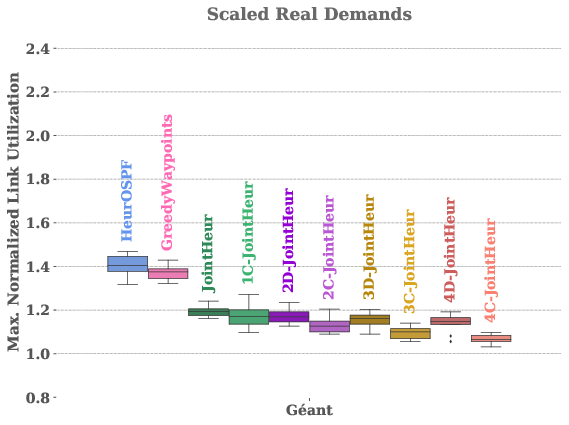
\includegraphics[width=\linewidth]{assets/g1rep0.png}
\end{figure}
\begin{figure}
  \centering
  \caption{Replikation fig. 2 in Simulation Umgebung}
  \label{fig:g01r}
  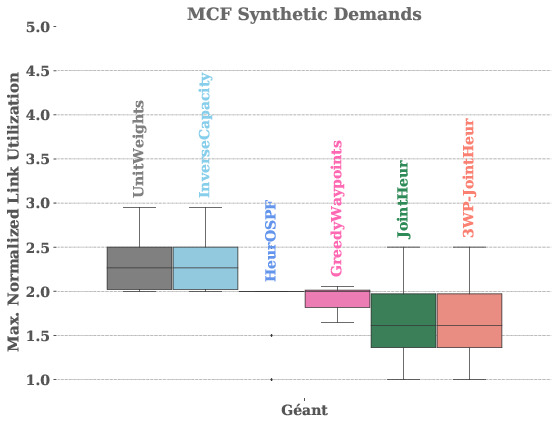
\includegraphics[width=\linewidth]{assets/g1rep1.jpg}
\end{figure}
\begin{figure}
  \centering
  \caption {Replikation fig. 3 in Simulation Umgebung}
  \label{fig:g02r}
  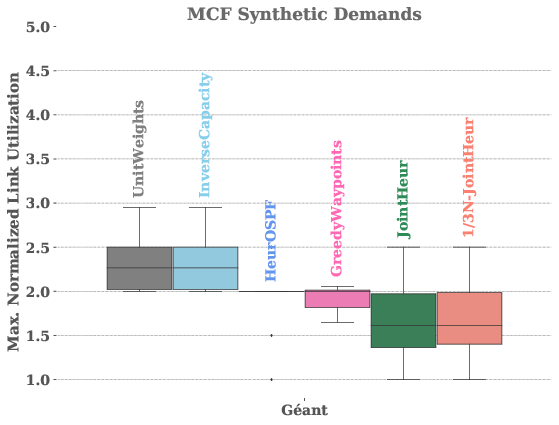
\includegraphics[width=\linewidth]{assets/g1rep2.png}
\end{figure}
Weiterhin entsprechen unsrer so erhobenen Resultate der Datenbasis der Gruppe, somit können wir der Gruppe mit guten Gewissen die Replizierbarkeit des ersten Experimentes attestieren.
\subsubsection{Nanonet}
Angelehnt an die Replizierung des Papers, hatte die Gruppe ihr Repository derartig präpariert, sodass das mehrmalige Ausführen des Experiments über die Namen der drei Algorithmen ein Resultat erbrachte. Es sei Anzumerken das hier natürlich vorausgesetzt wurde, das alle Abhäingkeiten installiert waren und die allgemeinen postulierten Startbedingungen des Skriptes eingehalten wurden.
\begin{figure}
  \centering
  \caption{Replikation Nanonet}
  \label{fig:g02r}
  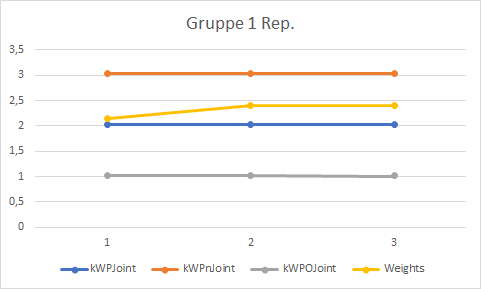
\includegraphics[width=\linewidth]{assets/g01r.png}
\end{figure}
Auch hier kann der Gruppe wieder attestiert werden, dass Ihre Ergebnisse nachweisbar sind, denn unsre Resultate decken sich soweit mit der Datenbasis der Gruppe. Auch die offerierten Experimente wirken schlüssig um die präsentierten Algorithmen der Gruppe zu simulieren. 
\section{Unsere eigenen Algorithmen}
\subsection{RandomWaypoints}
\subsubsection{Idee \& Algorithmus }
Unser erster Algorithmus nennt sich "RandomWaypoints" und ist eine Abänderung des "DemandFirstWaypoints" aus dem Paper \cite{10.1145/3485983.3494846}. Um den RandomWaypoints zu verstehen muss erst ein Einblick in DemandFirstWaypoints geschehen. In diesem Algorithmus wird in einer äußeren For-Schleife über jeden Demand iteriert. Innerhalb dieser Schleife folgt eine weitere Schleife, welche über jeden Knoten iteriert, der nicht Source oder Target des jeweiligen Demands ist. Der Knoten der jeweiligen Iteration stellt einen Wegpunkt für den jeweiligen Demand dar und wird dementsprechend erst einmal in der Flow-Map eingesetzt und geprüft ob der Weg, über Source nach Wegpunkt und Wegpunkt nach Target, die Maximum Link Utilization (MLU) verbessert, nach unserere Zielfunktion verringert. Falls dem so ist, wird dieser Wegpunkt als "noch" bester Wegpunkt gespeichert und falls es noch einen besseren Wegpunkt gibt in folgenden Iterationen der inneren For-Schleife abgelöst und überschrieben. Durch diesen Algorithmus werden Pfade, welche ohne einen Wegpunkt eine starke Auslastung haben, entlastet. RandomWaypoints handelt ähnlich wie DemandFirstWaypoints, jedoch ist es unser Ziel gewesen den Pool , aus dem die Wegpunkte genommen werden, um geprüft zu werden ob sie die Maximum Link Utilization verbessern, zu verringern und daraus folgend die Rechenzeit zu verringern. Die Idee dabei ist es für jeden Demand eine bestimmte Anzahl an zufälligen Wegpunkten herauszufiltern. Dann wird geprüft ob einer der Wegpunkte die Maximum Link Utilization verbessert und speichern diesen dann, falls dieser die MLU verbessert. Folgend ist ein Pseudocode gegeben, welcher aus der konkreten Python Implementierung \cite{repository-project1} zu entnehmen ist.

\begin{algorithm}
\caption{RandomWaypoints}
\begin{algorithmic}[1]
\FOR{$demand \; in \; demand\_list$} 
\STATE $waypointCount = x$
\STATE $randomList = \; Liste \; aus \; "x" \; zufälligen \; Zahlen$
\WHILE{$ein \; Element \; aus \; randomList  \; Source \; / \; Target \; ist$}
\STATE $randomList = \; Liste \; aus \; "x" \; zufälligen \; Zahlen$
\ENDWHILE
\FOR{$waypoint \; in \; randomList$}
\STATE $wenn \; waypoint \; MLU \; verbessert \; dann \; speichern$
\ENDFOR
\ENDFOR
\end{algorithmic}
\end{algorithm}

Der Algorithmus geht jeden Demand in der äußeren For-Schleife durch. Es gibt eine Variable WaypointCount mit der man die Anzahl an zufälligen Wegpunkten festlegt, diese darf jedoch nicht größer als die Gesamtanzhal an Nodes sein. Dann wird eine Liste randomList initialisiert in der waypointCount-viele verschiedene zufällige verschiedene Zahlen gespeichert werden. Jene werden benutzt um auf die Node List zuzugreifen als Indizes. Darauf folgt eine while-Schleife um Listen zu filtern die als zufälligen Wegpunkt den Source oder Target des Demands der Iteration haben. Am Ende ist eine zweite innere For-Schleife die für jeden der Wegpunkte prüft, ob er die MLU verbessert. Genau so wie beim GreedyWaypoints aus dem Paper \cite{10.1145/3485983.3494846}.

\subsection{DemandShortestPath}
Auch unser zweiter Algorithmus, getauft auf den Namen "Demand Shortes Path", ist wieder eine Modifikation des "Demand First Waypoint" aus dem Paper \cite{10.1145/3485983.3494846}. Die Zielsetzung der Modifikation bestand darin die Laufzeit gegenüber "Demand First Waypoint" zu optimieren und dabei möglichst nicht die MLU zu verschlechtern.\\
Betrachten wir als nächstes die Idee, dafür müssen wir allerdings erstmals etwas abschweifen, denn die Idee substanziiert sich auf der Funktionsweise von Demand First Waypoint. Grob gesagt, testet der besagte Algorithmus für jeden Demand alle Knoten im Netzwerk und wählt dabei den vermeintlich besten Knoten aus, der als Wegpunkt den vorteilhaftesten Einfluss auf die MLU hat. Offensichtlich führt dieses Vorgehen zwar zu einem passablen Ergebnisse, allerdings erscheint es nicht besonders opportun alle Knoten zu testen wenn auch die Laufzeit von Relevanz ist.
Daraus ergibt sich die Idee, die Menge der Knoten, die als Wegpunkt für einen Demand in Frage kommen einzuschränken um so die Laufzeit des Algorithmus zu verringern. Augenscheinlich ist die Wahl dieser Menge nicht ganz trivial, denn eine ungünstige Selektion, gerade mit z.B weit entfernten Wegpunkten, führt möglicherweise zu einem sehr schlechten Ergebnis. Und so war die Idee geboren, nur die Wegpunkte entlang eines kürzesten Weges zu betrachten.
\begin{algorithm}[hbt!]
\caption{Demand Shortest Path}\label{alg:cap}
\begin{algorithmic}[1]
    \REQUIRE {$Graph \; G$}
    \FORALL{$(s,t) \in Demands$} 
        \STATE $SPLN \gets Dijkstra(G,s,t)$
        \STATE $pw \gets \{ \}$
        \FORALL {$m \in SPLN$} 
            \FORALL{$b \in adj(m)$} 
                \STATE $pw \gets pw \cup \{b\}$
            \ENDFOR
        \ENDFOR
        \STATE $demandFirtsWaypoint(pw)$
    \ENDFOR
\end{algorithmic}
\end{algorithm}
Die Funktionsweise stellt sich wie folgt da, als erstes wird zu einem Demand ein kürzester Weg berechnet, anschließend werden alle Knote, die adjazent zu den Knoten auf dem Weg sind, in die Menge der potenziellen Wegputzte eingetragen. Nachfolgend wird der demand First Waypoint mit der beschriebenen Menge aufgerufen.

\subsection{IndependentPathsWaypoints}
Der Algoritmus IndependentPathsWaypoints (IPW) versucht die verschieden Demands durch ein Netzwerk so auf das gesamte Netzwerk zu verteilen, dass keine einzelne Verbindung im Netzwerk überlastet wird. 
Dazu werden verschiedene Demands, wenn möglich, über verschiedene Wege durch das Netzwerk geleitet. 
IPW geht dabei nach einem Greedy Ansatz vor. 
Um unnötige Berechnungen zu verhindern, werden für die Wege nur die $n$ kürzesten Pfade von Quelle eines Demands zu dessen Ziel in betracht gezogen.
Die kürzesten Wege werden mit dem Algorithmus von Dijkstra \cite{10.1007/BF01386390} berechnet.
Wir haben dabei eine vorgefertigte Implementierung "$all\_pair\_shortest\_path$" aus der Python-Bibliothek NetworkX \cite{networkx} verwendet. 

Für jeden der berechneten $n$-kürzesten Pfade werden nun Wegpunkte eingetragen und mit Hilfe der Simmulationsumgebung \cite{python-simmulation} die MLU berechnet.
Ist diese besser als eine zuvor berechnete MLU so wird dieser Weg genommen, anderenfalls wird der Weg verworfen.
Durch dieses Vorgehen ist sichergestellt, das wir für jeden Demand den bestmöglichen Weg, unter Berücksichtigung bereits vorhandener Demands, wählt.
Es kann nun passieren das ganz kleine Demands dafür sorgen, dass ein großer Demand über einen "Umweg" geleitet wird.
Dies umgehen wir indem wir die Demands priorisieren. 
Dazu werden die Demands nach ihrer Größe sortiert, und die Berechnung der Wegpunkte beginnt mit dem größten Demand.
Der Pseudocode von IPW ist  in \ref{pseudo:iwp} angegeben.

\lstset{
  numbers=left,
  stepnumber=1,    
  firstnumber=1,
  numberfirstline=false
}
\begin{lstlisting}[language=Python, caption={Independet Paths Waypoints}, label=pseudo:iwp]
IndependetPathsWaypoints (Graph, Demands, n)
best_objective = utilization()
paths[] = []
FOR demand in Demands do:
    src, dest = demand
    best_path = None
    i = 0
    FOR path in all_shortest_path(Graph, src, dest) do:
        if i > n
            break
        else
            i++
        
        if len(path) == 2
            best_path = path
            break
        else
            add all nodes on path as waypoints
            objective = untilization()
            
            if objective > best_objetive
                best_path = path
                best_obejctive = objetive
    append(paths, best_path)
    ENDFOR
ENDFOR
return best_objetive, paths
    

\end{lstlisting}




\section{Simulation in Python}
In dem folgenden Abschnitt wollen wir uns jeweils mit der Simulation der einzelne Algorithmen auseinandersetzen.

\subsection{\textbf{RandomWaypoints}}

In Fig. \ref{fig:random-mlu-10w-abilene} ist eine Auswertung bezüglich des Objectives MLU und 10 Wegpunkten gegeben. Dazu muss gesagt werden, dass das Netz vergleichsweise sehr klein ist zu den anderen vorgegebenen Netzen. Bei dem hellblauen Boxplot rechts handelt es sich um RandomWaypoints, welcher verglichen wird mit DemandShortestPath (lila) , IndependentPathsWaypoints (gelb) , GreedyWaypoints (rosa) und InverseCapacity (links , marineblau). Man kann erkennen, dass der Boxplot des RandomWaypoints nicht allzu unterschiedlich ist zu dem Boxplot des GreedyWaypoints, was schließlich auch die Intention unserer Idee war. \\
Den zweiten Teil unserer Idee, nämlich die Verbesserung der Laufzeit kann man in Fig. \ref{fig:all-mlu-time-plot} genauer betrachten. Hier wird das  Objective (MLU) auf der X-Achse und die Zeit, die die Algorithmen brauchen, auf der Y-Achse abgebildet. Der Fig. \ref{fig:all-mlu-time-plot} kann man entnehmen, dass RandomWaypoints (hellblau ca. (1.35, 0.050)) vergleichsweise wenig Zeit benötigt jedoch das Objektiv darunter leidet. Pauschal lässt sich aussagen, dass je weniger Zeit der Algorithmus braucht, desto weniger Wegpunkte  werden getestet, desto geringer ist die Wahrscheinlichkeit den richtigen Wegpunkt zu finden, daher auch die schlechtere MLU.\\ 
Den Effekt den die Anzahl an Wegpunkten hat, kann in der folgenden Fig. \ref{fig:random-n-points-efect} genauer betrachtet werden. Links 
ist ein Plot zu sehen, bei dem RandomWaypoints mit 3 Wegpunkten, ausgeführt wurde und rechts mit 10 Wegpunkten. Durch genaueres Betrachten kann man sehen dass die Whisker auf der gleichen Höhe sind, dagegen ist die Box bei den 3 Wegpunkten nach oben geschoben, was bezüglich der MLU bedeutet, dass es schlechter ist. Die rote Linie zeigt wo sich das untere Quantil des 10-Wegpunkte-Durchlaufs im 3-Wegpunkte-Durchlauf einordnet. Es könnte jedoch auch dazu kommen, dass eine Ausführung mit weniger Wegpunkten besser ist, als eine mit mehr Wegpunkten, aufgrund der Randomisierung. Daher ist RandomWaypoints nicht konstant gut und wird auch nie besser als DemandFirstWaypoints, da er nicht mehr, als alle Nodes, als Wegpunkt testen kann.

\subsection{IndependentPathsWaypoints}
In Abbildung \ref{fig:mlu-abilene-geant} ist die MLU von IPW (Gelb)  auf den Topologien Abilene und Gèant dargstellt.
Da wir nur beschränkte Rechen-ressourcen zur Verfügung haben erfolgt die Auswertung hier nur auf zwei sehr kleinen Topologien.
Es ist klar zu erkennen, dass IWP kein optimales Routing für das Netzwerk findet.
Die anderen entwickelten Algorithmen, außer das Gewichten der Kanten nach ihrer inversen Kapazität, haben einen bessere MLU als IWP.
Auch kann man einen Zusammenhang zwischen IWP und InverseCapacity sehen. In  der Topologie Abilene erreicht InverseCapacity mit einer MLU von ca. 1.2 einen recht guten Wert.
Auch IPW kommt hier mit ca. 1.3 auf einen guten Wert.
In der Topologie Gèant ist IPW mit einer MLU von 2.3 weit hinter den anderen Algorithmen, InverseCapacity ist noch weiter abgeschlagen mit einer MLU von 2.5.
Dieser Effekt ist durchaus auch in anderen Topologien zu sehen, wenngleich wir dies aufgrund unserer beschränkten Rechen-resourcen und Zeit wir dies nicht fuer alle Topologien überpruefen konnten. 
Wenn man sich die Arbeitsweise der Algorithmen anschaut ist dieser Zusammenhang durchaus plausibel. 
Sowohl IPW als auch InverseCapacity nutzen die Kapzität der Kanten um die Kantengewichtungen festzulegen. 
IPW versucht danach zusätzlich noch die Demands über mehrere Wege zu verteilen, was zu dem leichten Vorteil bei Gèant führt.

Betrachtet man unsere zweite Auswertung nach der Ausführungszeit in \ref{fig:all-mlu-time-plot}, die die Algorithmen jeweils benötigen, 
so stellt man fest, dass IPW die Rechenzeit im Vergleich zu GreedyWaypoints durchaus reduziert. 
Im Vergleich mit unseren anderen Algorithmen ist IPW der zweit schnellste.

Der IPW Algorithmus ist ein tradeoff zwischen schneller Rechenzeit und einer kleinen MLU. 
Er kann genutzt werden in Netzen die sich öft ändern, da neue Routen schnell berechnet werden können. 
Dafür ist die MLU leider nicht so gut wie bei anderen Algorithmen.

\begin{figure}
  \centering
  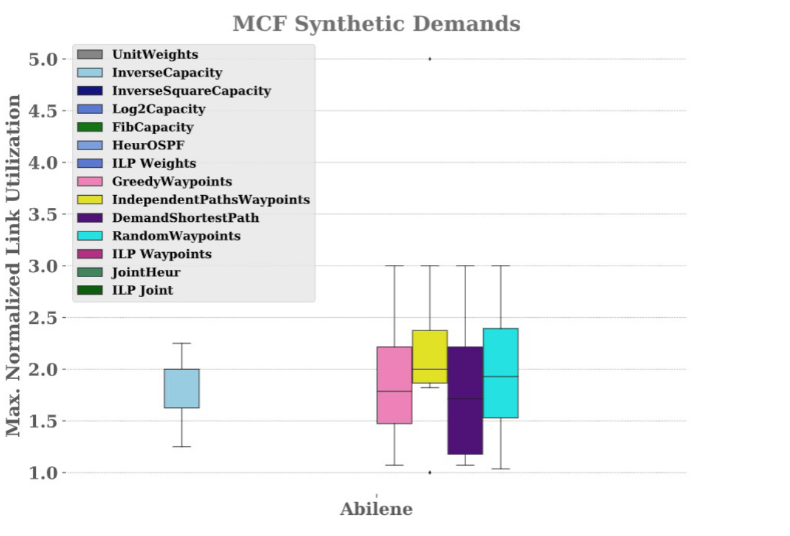
\includegraphics[width=\linewidth]{assets/mluwaypoints.png}
  \caption{RandomWaypoints MLU Ergebnisse mit 10 Waypoints}
  \label{fig:random-mlu-10w-abilene}
\end{figure}

\begin{figure}
  \centering
  \caption{Ausführungszeit mit MLU}
  \label{fig:all-mlu-time-plot}
  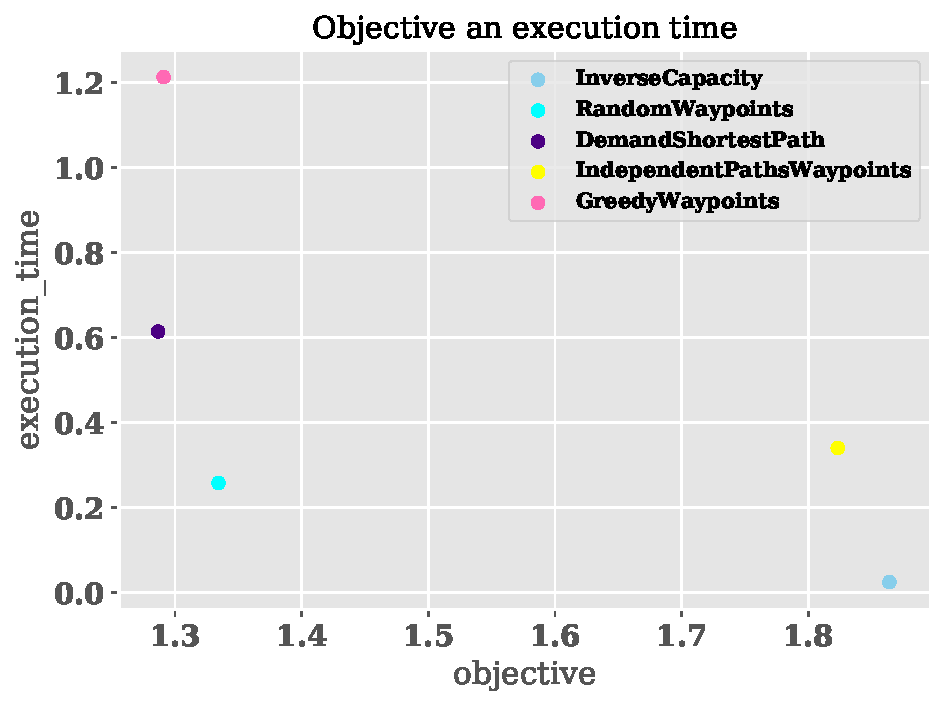
\includegraphics[width=\linewidth]{assets/execution_time.pdf}
\end{figure}

\begin{figure}
  \centering
  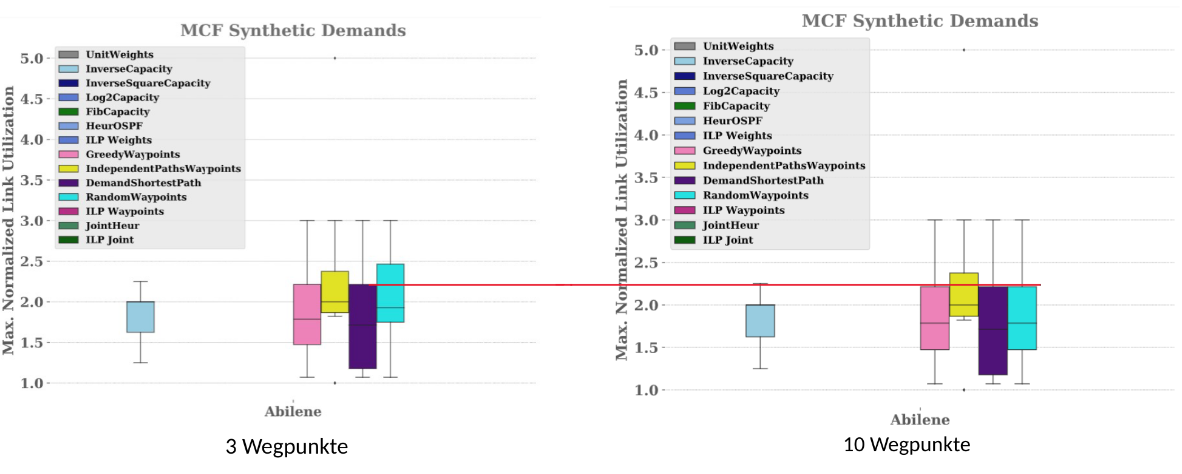
\includegraphics[width=\linewidth]{assets/3vs10randomWP.png}
  \caption{Effekt von Anzahl an Wegpunkten auf MLU}
  \label{fig:random-n-points-efect}
\end{figure}

\subsection{\textbf{DemandShortestPath}}
In Abbildung \ref{fig:mlu-abilene-geant} ist DemandShortestPath (DSP) in lila dargestellt, es ist schön zu erkennen, dass das Korelat von Greedy Waypoint (Pink) nur marginale Differenzen zu DPS aufweist. Damit ist die erste postulierte Prämisse, dass sich die Modifikation möglichst nicht negativ auf die MLU auswirkt erfüllt. Ein entsprechendes Resultat konnte auch bei größeren Topologien beobachtet werden. Für sich genommen wäre das auch schon ein Erfolg, allerdings möchte wir uns nun als nächstes mit der Rechenzeit beschäftigen, die als zweite formulierte Prämisse des Entwurfs eine Verbesserung erzielen sollte. Beachte dazu \ref{fig:all-mlu-time-plot}, augenscheinlich ist die Rechenzeit des Greedy Waypoint grob um einen Faktor 2 größer, dieses Ergebnis scheint auch bei größeren Topologien zuzutreffen. Dazu sei angemerkt, dass sich relativ trivial Topologien konstruieren lassen, wo die Laufzeit von DSP keine oder nur ein geringen Vorteil bietet, aber sie sollte auch niemals signifikant schlechter werden können, denn eine unbeschränkte Testmenge entspricht Greedy Waypoint mit konstanten Overhead.
Diese trifft allerdings nicht auf die Auswirkung auf die MLU zu. Es lässt sich auch hier relativ trivial eine Topologie zu konstruieren, wo ein opportuner Wegpunkt außerhalb der Testmenge von DSP liegt, dennoch innerhalb der Menge von Greedywaypoint. Abschließend suggeriert die Bilanz der erhobenen Daten aber durchaus eine vorteilhafte Auswirkung auf die Rechenzeit über die meisten Topologien, doch wie beschrieben mit dem Risiko einer negativen Beeinflussung auf die MLU. Dieses Zielkonfikt scheint aber vertretbar.

\begin{figure}
    \centering
    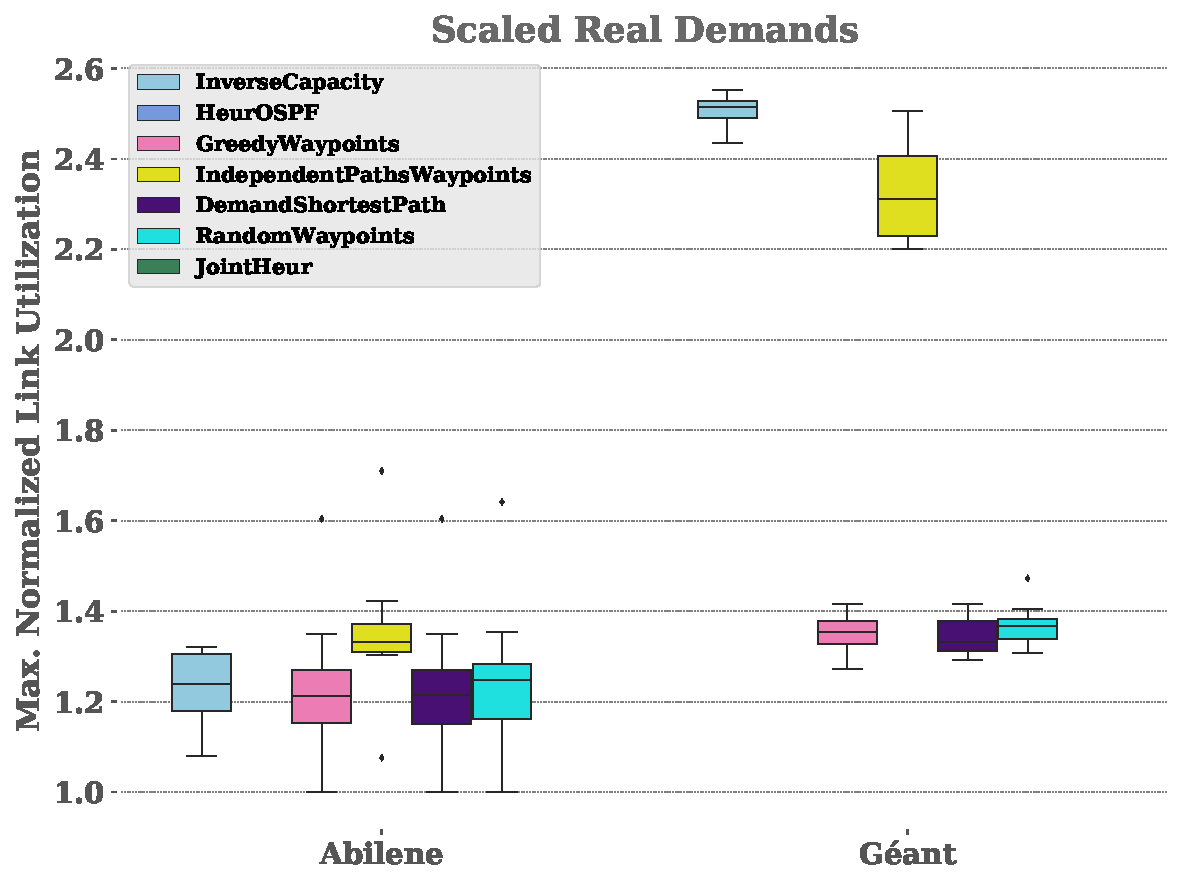
\includegraphics[width=\linewidth]{assets/real_demands-abilene-geant.pdf}
    \caption{MLU auf den Topologien Albile und Gèant}
    \label{fig:mlu-abilene-geant}
\end{figure}



\section{Evaluation in Nanonet}
Zu jedem unserer Algorithmen aus dem Projekt 1, haben wir jeweils eine Topologie entworfen die wir im Nanonet-Simulationsframework \cite{repository-project2} darauf getestet haben. Dazu erläutern wir die Gründe für die Entscheidung der Wahl dieser Topologien, wie wir diese modelliert haben und zu welchen Ergebnissen wir gekommen sind.

\subsection{RandomWaypooint}
Da dieser Algorithmus auf der Randomisierung basiert, sind wir auch randomisierend bei der Erstellung der Topologie dessen vorgegangen. Zunächst haben wir eine zufällige Anzahl an Knoten und Kanten gewählt. Daraufhin wurden per Hand die Kanten zwischen den Knoten eingesetzt so, dass jeder Knoten mindestens einen Nachbarn hat. Die Erstellung der Demands verlief ähnlich, denn deren Gewichte und Wegpunkte wurde auch mithilfe der Randomisierung bestimmt. Unser Ziel war es möglichst viele Faktoren, die bei der  Erstellung einer Topologie eine Rollen spielen, zu randomisieren. \\
\textbf{Ergebnisse .}
In Fig.  \ref{fig:weights-vs-random-mlu-plot} ist ein Plot der Ergebnisse von Weights (in rot) und RandomWaypoints (in blau) zu sehen. Dabei können diese gegeneinander in Bezug gesetzt werden in diesem Fall, da beide für die gleiche Topologie und den gleichen Demands simuliert wurden. Die Änderung, die RandomWaypoints an der Topologie noch vorgenommen hat, ist dass es bei den Demands noch einen zufälligen Wegpunkt gibt, den es bei der Weights Topologie zuvor nicht gab. Man kann erkennen, dass RandomWaypoints unter dieser Auswahl an Wegpunkten nahezu in jedem Punkt besser ist als Weights , da der Boxplot unter dem Minimum des Weights Plots ist. Das ist aber nur in diesem Fall so, es könnte auch eine schlechtere Auswahl an Wegpunkten geschehen und der Plot würde sich dann auch dementsprechend in den höheren MLU Bereich bewegen. 

\begin{figure}
  \centering
  \caption{Weights (rot) und RandomWaypoints (blau) unter MLU}
  \label{fig:weights-vs-random-mlu-plot}
  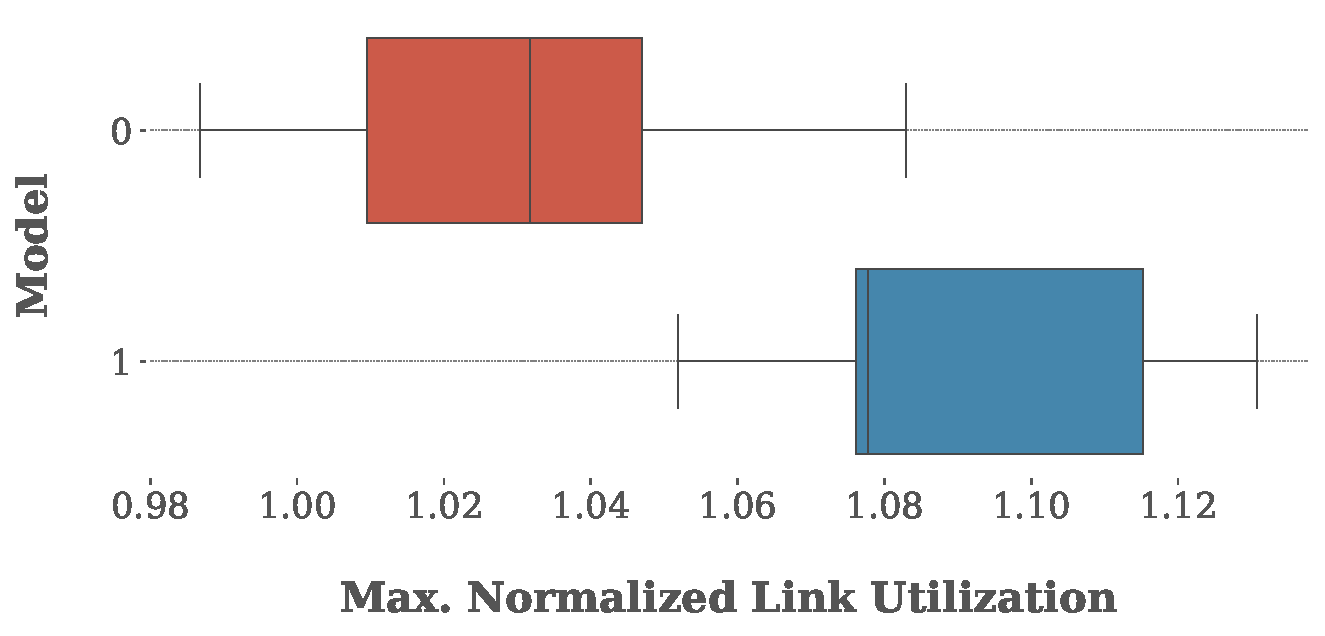
\includegraphics[width=\linewidth]{assets/weight_random.pdf}
\end{figure}
\begin{figure}
  \centering
  \caption{Weights (rot) und IndependentPathsWaypoints (blau) unter MLU}
  \label{fig:weights-iwp-nanonet}
  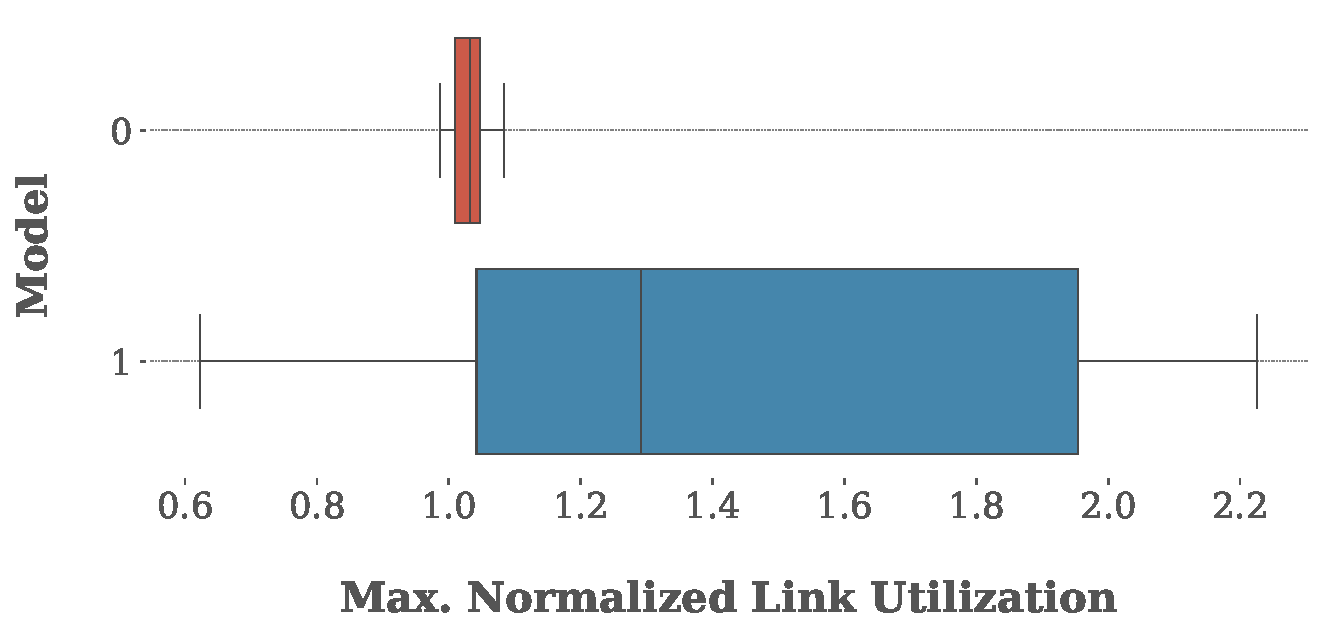
\includegraphics[width=\linewidth]{assets/weight_ipw.pdf}
\end{figure}

\subsection{DemandShortestPath}
Desgleichen wurde auch Demand Shortes Path mit dem Alogorimus "Weights" verglichen, allerdings haben wir nicht die mitgelieferte Topologie verwendet, sondern eine eigene entworfen. Diese sollte ein potenzielles reales Netz porträtieren, dennoch aber einfach genug sein, sodass eine Übertragung ins Simulations-Framework und eine anschließende manuelle Anfertigung eines Experimentes im Nanonet möglich war. 
\begin{figure}
  \centering
  \caption{Nanonet DSP}
  \label{fig:figNanonetDSP}
  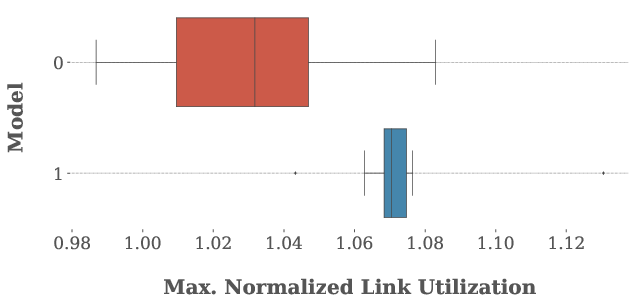
\includegraphics[width=\linewidth]{assets/figNanonetDSP.png}
\end{figure}
Das anschließenden Ergebnis war allerdings ehr ernüchternd, "Weights" liefert wenn auch marginal gegenüber DSP konstant bessere Ergebnisse. Das lässt natürlich den Schluss zu, dass es sich bei dem Experiment um eine Fehl-Konfiguration handelt oder das gerade die Topologie ungünstig gewählt ist. Aber wahrscheinlich wichtiger ist das Resultat, dass die Labor Bedingen des Simulation Frameworkes nicht immer die Realität abbilden müssen. Und vielleicht ist es auch ein Erfolg das sich das Ergebnis nicht nennenswert verschlechtert hat, allerdings ist vermutlich eine reale Anwendung des DSP Algorithmus nur unter sehr eingeschränkten Konditionen wenn überhaupt opportun.
\subsection{IndependentPathsWaypoints}
Wir haben IPW im Nanonet mit dem Algorithmus "Weights" verglichen. Dazu haben wir die Topologie von Weigths um Wegpunkte erweitert.
Um die Wegpunkte zu bestimmen, haben wir die Topologie, die Weights in Nanonet benutzt, mit IPW in der Python- simualationsumgebung ausgeführt und die gewählten Wegpunkte ausgegben.
Diese haben wir dann manuell in das Nanonet übertragen.
Die "Weights" Topologie hatte zu beginn nur einen Demand, wir haben diese um einen zweiten Demand erweitert da IPW mit nur einem Demand genau das gleiche Routing wie "Weights" durchführen würde.
In IPW werden nun beide Demands über verschiedene Wege geleitet. In "Weights" gehen beide über den gleichen Weg.
In Abbildung \ref{fig:weights-iwp-nanonet} kann man die Ergebnisse der Auswertung sehen.
Man sieht direkt, das IWP eine sehr große spanne an Werten hat. 
Dies liegt daran das wir beim Ausführen der Nanonet-Simualtion teilweise Probleme mit den Netzwerk-Namespaces hatten. 
Während in der Simulation waren manche virtuelle Nodes sporadisch nicht erreichbar, was dann zu Paketverlust geführt hat.
Im Moment konnten wir dem Problem aber noch keine Abhilfe schaffen.
Mann kann in dem Boxplot aber trotzdem abschätzen, dass IPW durchaus in der Lage ist die Demands besser zu verteilen als Weights dies kann.

Eine Auswertung nach der Rechenzeit konnten wir, da wir die Wegpunkte außerhalb des Nanonets berechnet haben, nicht vornehmen.
Da aber sowohl die Nanonet DSL sowie unsere Simmualtionsumgebung in Python geschrieben sind erwarten wir hier keine großen Unterschiede zu den Ergebnissen in \ref{fig:all-mlu-time-plot}.


\section{Recap}
\subsection{Comparision Python simulation and Nanonet}

Wenn man die Auswertungen unsere Algorithmen in der Python-simulation, mit der Topologie Abilene Abbildung \ref{fig:mlu-abilene-geant}, mit den Ergebnissen in der Simulation in Nanonet, Abildungen \ref{fig:weights-iwp-nanonet}, \ref{fig:weights-vs-random-mlu-plot} und \ref{fig:weights-vs-random-mlu-plot} vergleicht erkennt man folgendes:
\begin{itemize}
    \item In Abilenen ist der beste Algorithmus unter Betrachtung der MLU RandomWaypoints, darauf folgt DemandShortestPath und am ende der Liste folgt IndependetPathsWaypoints.
    \item In den Auswertungen mit Nanonet ist der beste Algorithmus unter betrachtung der MLU ebenfalls RandomWaypoints, gefolgt von DemandShortestPath und IndependentPathsWaypoints.
\end{itemize}
Daraus lässt sich schließen, dass die Python-Simmulationumgebung \cite{python-simmulation} durchaus geeignet ist um die Effektivität von Routingalgorithmen in
zumindest softwarebasierten Netzwerken festzustellen.
Dies insofern erfreulich, da es wesentlich einfacher ist die Algorithmen in der Python-Simulationsumgebung zu integrieren als in Nanonet.
Neue algorithmische Ideen könnnen also einfach und Zeiteffektiv in der Python-Simmulationsumgebung getestet werden. 
\section{Zusammenfassung}
Abschließend kann man sagen, dass wir den Entwicklungsprozess eines Routingalgorithmus einmal durchgespielt haben. Von der theoretischen Entwicklung im Python Simulationsframework bis zur praktischen Anwendung im Nanonet. Alle unserer Algorithmen haben sich als umsetzbar erwiesen, wobei IPW aufgrund seiner schlechten Performance unter der Zielfunktion MLU in der Praxis nicht zu empfehlen ist.
\section{Ausblick}
Für die Zukunft wäre es opportun das Nanonet Framework um weitere Funktionen zu erweitern, damit man Daten wie z.B. die Rechenzeit zur Bestimmung der Routingpfade erheben kann.
Wir könnten dann unsere Algorithmen in Nanonet direkt implementieren und müssten sie nicht erst simulieren.
Damit können wir ergründen ob die, in der Python Simulation, festgestellten Rechenzeitverbesserungen auch wirklich in Nanonet festellbar sind.

Die große Streuung von IPW im Nanonet sollte weiter untersucht werden, da diese durch einen Implementations-fehler des Algorithmus im Nanonet-Framework bedingt sein können.

Weiterhin interessant ist es auch zu untersuchen ob Randomisierte Algorithmen in gängiger Netzwerk-Hardware überhaupt implementierbar sind.

Ebenfalls sinnvoll erscheint eine weitere Untersuchung der drei Algorithmen in echter Hardware.
Da uns nur sehr beschränkte Computerresourcen zur Verfügung standen konnten wir die Algorithmen immer nur in kleinen Netzwerken testen.
Es wäre interessant diese auch in großen Netzen zu evaluieren.

%%\begin{description}
%%\item[\texttt{sidebar}:]  Place formatted text in the margin.
%%\item[\texttt{marginfigure}:] Place a figure in the margin.
%%\item[\texttt{margintable}:] Place a table in the margin.
%%\end{description}



%%
%% The next two lines define the bibliography style to be used, and
%% the bibliography file.
\bibliographystyle{ACM-Reference-Format}
\bibliography{bibliography}


%%
%% If your work has an appendix, this is the place to put it.
\appendix

\end{document}
\endinput
%%
%% End of file `sample-acmtog.tex'.
